\documentclass[aspectratio=169]{beamer}

% Shared Beamer settings for Applied Machine Learning lectures (UPES).
% Keep this file free of \documentclass to allow reuse via \input.

% Allow lecture sources to use shared theme/assets without copying them into each lecture folder.
% NOTE: These paths are relative to `Unit-xx/Lecture-yy/latex/` (and `Lab/Experiment-xx/latex/`).
\makeatletter
\def\input@path{{../../../_shared/}{../../../_shared/UPES-Beamer-Theme/}}
\makeatother

\usetheme{UPES}
\setbeamertemplate{navigation symbols}{}

\usepackage{amsmath}
\usepackage{amssymb}
\usepackage{booktabs}
\usepackage{graphicx}
\usepackage{hyperref}
\usepackage{xcolor}
\usepackage{listings}

% Code listings (Python-oriented for this subject).
\lstset{
  language=Python,
  basicstyle=\ttfamily\small,
  keywordstyle=\color{blue},
  commentstyle=\color{gray},
  stringstyle=\color{teal},
  showstringspaces=false,
  columns=fullflexible,
  breaklines=true
}

\usepackage{tikz}
\usetikzlibrary{arrows.meta,positioning,shapes.geometric,calc,fit,backgrounds}

% Per-slide source line (references shown on the slide itself).
\newcommand{\slidesources}[1]{%
  \vfill
  {\tiny\color{gray}\raggedright\sloppy\parbox{\linewidth}{Sources: #1}\par}%
}

% Unit-wise source strings for this subject (used by slides/notes).
% Path is relative to the lecture `latex/` folder (the compilation CWD).
% Source strings for Applied Machine Learning (CSAI2017P) — used by slides + notes.
% Prescribed texts and reference books are taken from the course syllabus.
% Support texts are the author-hosted open-access editions:
%   statlearning.com            (ISL with Python)
%   probml.github.io/pml-book   (Murphy, Probabilistic Machine Learning)
%   d2l.ai                      (Dive into Deep Learning)
%   mml-book.github.io          (Mathematics for Machine Learning)

\newcommand{\AMLRepoURL}{https://github.com/tali7c/Applied-Machine-Learning}

% --- prescribed -------------------------------------------------------------
\newcommand{\AMLPrescribed}{%
M\"uller and Guido, \textit{Introduction to Machine Learning with Python}, O'Reilly, 2016.;%
Bishop, \textit{Pattern Recognition and Machine Learning}, Springer, 2006.;%
Murphy, \textit{Machine Learning: A Probabilistic Perspective}, MIT Press, 2012.;%
Han, Kamber and Pei, \textit{Data Mining: Concepts and Techniques} (3e), Morgan Kaufmann, 2012.%
}

% --- unit-wise ---------------------------------------------------------------
\newcommand{\AMLUnitISources}{%
M\"uller and Guido, \textit{Introduction to Machine Learning with Python}, Ch. 1.;%
Bishop, \textit{Pattern Recognition and Machine Learning}, Ch. 1.;%
Murphy, \textit{Probabilistic Machine Learning: An Introduction}, MIT Press, 2022, Ch. 1.;%
Mitchell, \textit{Machine Learning}, McGraw Hill, 1997, Ch. 1.;%
Scikit-learn documentation, accessed 2026-08-04.%
}

\newcommand{\AMLUnitIISources}{%
Bishop, \textit{Pattern Recognition and Machine Learning}, \S1.5, \S4.3, \S7.1.;%
Zhang, Lipton, Li and Smola, \textit{Dive into Deep Learning}, \S3.4.;%
Shalev-Shwartz and Ben-David, \textit{Understanding Machine Learning}, Ch. 15.;%
Murphy, \textit{Probabilistic Machine Learning: An Introduction}, Ch. 5.%
}

\newcommand{\AMLUnitIIISources}{%
Zhang, Lipton, Li and Smola, \textit{Dive into Deep Learning}, Ch. 12 (Optimization Algorithms).;%
Deisenroth, Faisal and Ong, \textit{Mathematics for Machine Learning}, Ch. 7.;%
Kingma and Ba, ``Adam: A Method for Stochastic Optimization,'' ICLR 2015.;%
Ruder, ``An overview of gradient descent optimization algorithms,'' arXiv:1609.04747, 2016.%
}

\newcommand{\AMLUnitIVSources}{%
Han, Kamber and Pei, \textit{Data Mining: Concepts and Techniques} (3e), Ch. 3.;%
M\"uller and Guido, \textit{Introduction to Machine Learning with Python}, Ch. 3--4.;%
James, Witten, Hastie, Tibshirani and Taylor, \textit{An Introduction to Statistical Learning with Python}, Ch. 5--6, 12.;%
Scikit-learn documentation (preprocessing, model selection), accessed 2026-08-04.%
}

\newcommand{\AMLUnitVSources}{%
James et al., \textit{An Introduction to Statistical Learning with Python}, Ch. 3--6.;%
Bishop, \textit{Pattern Recognition and Machine Learning}, Ch. 3.;%
Deisenroth, Faisal and Ong, \textit{Mathematics for Machine Learning}, Ch. 9.;%
M\"uller and Guido, \textit{Introduction to Machine Learning with Python}, \S2.3.%
}

\newcommand{\AMLUnitVISources}{%
Han, Kamber and Pei, \textit{Data Mining: Concepts and Techniques} (3e), Ch. 8--9.;%
James et al., \textit{An Introduction to Statistical Learning with Python}, Ch. 8--9.;%
Bishop, \textit{Pattern Recognition and Machine Learning}, Ch. 4--5, 7, 14.;%
Zhang et al., \textit{Dive into Deep Learning}, Ch. 5.%
}

\newcommand{\AMLUnitVIISources}{%
Han, Kamber and Pei, \textit{Data Mining: Concepts and Techniques} (3e), Ch. 10.;%
James et al., \textit{An Introduction to Statistical Learning with Python}, Ch. 12.;%
M\"uller and Guido, \textit{Introduction to Machine Learning with Python}, \S3.5.;%
Ester, Kriegel, Sander and Xu, ``A density-based algorithm for discovering clusters (DBSCAN),'' KDD 1996.%
}

\newcommand{\AMLLabSources}{%
M\"uller and Guido, \textit{Introduction to Machine Learning with Python}, companion notebooks.;%
McKinney, \textit{Python for Data Analysis} (3e), O'Reilly, 2022.;%
Scikit-learn user guide, accessed 2026-08-04.;%
Matplotlib and Seaborn documentation, accessed 2026-08-04.%
}



\graphicspath{{../figures/}{../images/}{../../../_shared/}{../../../_shared/UPES-Beamer-Theme/}}

\title[Applied Machine Learning]{Applied Machine Learning}
\subtitle{Unit 04 -- Lecture 07: Splitting, Validation and Imbalance}
\author{Tofik Ali}
\institute{School of Computer Science, UPES Dehradun}
\date{Autumn 2026}

% ---- a compact "output" block so code and its result sit together ----------
\lstdefinestyle{outblk}{
  basicstyle=\ttfamily\scriptsize\color{black!75},
  backgroundcolor=\color{black!5}, frame=leftline, framerule=2pt,
  rulecolor=\color{black!30}, breaklines=true, columns=fullflexible,
  keepspaces=true,   % several outputs below are aligned tables
  language={},       % printed output is not Python: do not syntax-highlight it
  xleftmargin=4pt, aboveskip=1pt, belowskip=1pt, literate={-}{{-}}1}
\lstnewenvironment{outblk}{\lstset{style=outblk}}{}

\begin{document}

\UPESCoverFrame
\setcounter{framenumber}{0}

\begin{frame}
  \titlepage
  \begin{center}
    \footnotesize Splitting, cross-validation and imbalanced data\\[0.2em]
    \footnotesize Topic focus: \textbf{a score is an estimate, and every
    estimate has a spread}\\[0.2em]
    \footnotesize Repository: \texttt{\AMLRepoURL}
  \end{center}
  \slidesources{\AMLUnitIVSources}
\end{frame}

\begin{frame}{Quick Links}
  \centering
  \hyperlink{sec:split}{\beamerbutton{One split}}\hspace{0.4em}
  \hyperlink{sec:strategy}{\beamerbutton{Split strategies}}\hspace{0.4em}
  \hyperlink{sec:cv}{\beamerbutton{Cross-validation}}\hspace{0.4em}
  \hyperlink{sec:nested}{\beamerbutton{Tuning honestly}}\hspace{0.4em}
  \hyperlink{sec:imbal}{\beamerbutton{Imbalanced data}}\hspace{0.4em}
  \hyperlink{sec:summary}{\beamerbutton{Summary}}
\end{frame}

\begin{frame}{Agenda}
  \tableofcontents
\end{frame}

\begin{frame}[shrink=6]{How this lecture works}
  \begin{columns}[T]
    \begin{column}{0.48\textwidth}
      \begin{block}{Every idea appears twice}
        \begin{enumerate}
          \item \textbf{By hand} --- twelve rows split three ways, a
            $1000$-patient confusion matrix, two points and a straight line.
            Small enough to check on paper.
          \item \textbf{In code} --- the same arithmetic on real data, so you
            see that \texttt{StratifiedKFold} and \texttt{GroupKFold} do
            exactly that and nothing more.
        \end{enumerate}
      \end{block}
    \end{column}
    \begin{column}{0.48\textwidth}
      \begin{alertblock}{Commit before you look}
        Five slides ask you to predict a number before it is revealed. Write
        your guess down. Being wrong on paper is how the idea sticks.
      \end{alertblock}
    \end{column}
  \end{columns}
  \vspace{0.4em}
  \begin{center}
    \small The centrepiece: \textbf{the same three lines of code report
    $F_1 = 0.894$ or $F_1 = 0.113$}, depending on where you put one of
    them.
  \end{center}
\end{frame}

\begin{frame}[shrink=5]{Where we are}
  \begin{columns}[T]
    \begin{column}{0.47\textwidth}
      \begin{block}{Last lecture chose the columns}
        Scaling, encoding, PCA, selection. It ended on one measurement:
        \textbf{selecting features before splitting scored $0.8475$ on data
        made of coin flips}.
      \end{block}
      \begin{block}{That was a symptom}
        The disease is the \emph{split} --- what goes in it, when it happens,
        and what it is allowed to know.
      \end{block}
    \end{column}
    \begin{column}{0.49\textwidth}
      \begin{exampleblock}{Today's four questions}
        How reliable is a single held-out score? What if the rows are not
        independent? How many folds? And what do I do when one class is
        $1\%$ of the data?
      \end{exampleblock}
      \begin{alertblock}{One sentence to carry through}
        \small \textbf{Anything you learn from the data --- a mean, a
        category list, a feature subset, a hyper-parameter, a resampled
        row --- is part of the model, and belongs inside the loop.}
      \end{alertblock}
    \end{column}
  \end{columns}
\end{frame}

% =====================================================================
\section[One split]{A single train/test split}
\label{sec:split}

\begin{frame}[shrink=6]{What a held-out score is actually estimating}
  \begin{exampleblock}{}
    \centering\large
    The performance the model would have on \emph{new rows from the same
    source}.
  \end{exampleblock}
  \vspace{0.3em}
  \begin{columns}[T]
    \begin{column}{0.48\textwidth}
      \begin{block}{Why we hold anything out at all}
        \small A model can memorise. Training accuracy measures memory;
        held-out accuracy measures \emph{generalisation}. Every number you
        ever report should come from rows the model has not seen.
      \end{block}
    \end{column}
    \begin{column}{0.48\textwidth}
      \begin{alertblock}{But the held-out rows were also chosen at random}
        \small So the number you report is a \textbf{random variable}. It has
        a mean, and it has a spread, and \textbf{almost nobody reports the
        spread}.
      \end{alertblock}
    \end{column}
  \end{columns}
  \vspace{0.2em}
  \begin{center}\small
    \texttt{train\_test\_split(X, y, test\_size=0.25, random\_state=42)}
    --- the last argument is not a formality. It is a coin toss with your
    result on it.
  \end{center}
\end{frame}

\begin{frame}[shrink=6]{Four datasets, one seed --- and why this deck has sweeps}
  \begin{columns}[T]
    \begin{column}{0.48\textwidth}
      \begin{block}{One arbitrary seed}
        \small \texttt{np.random.default\_rng(0)},
        \texttt{random\_state=0}. Every listing that splits, shuffles or
        resamples shows it.
      \end{block}
    \end{column}
    \begin{column}{0.48\textwidth}
      \begin{block}{Three data seeds, kept}
        \small The $99{:}1$ problem, the $40$-patient study and the
        $600$-day series are \emph{defined} by their seeds, so those keep
        their own names and values.
      \end{block}
    \end{column}
  \end{columns}
  \begin{alertblock}{And a great many sweeps, on purpose}
    \small $500$ splits, $40$ shuffles, $20$ nested trials: these change seed
    every repetition, because \textbf{the spread across repetitions is the
    subject of this lecture}. Their seeds run \texttt{range(0, 500)},
    \texttt{range(0, 40)}, so the sweep still reproduces exactly. Run the code
    as written and every number here comes back --- except the seconds, which
    are labelled where they appear.
  \end{alertblock}
\end{frame}

\begin{frame}[shrink=8]{By hand: twelve rows, four held out}
  Twelve patients, nine healthy $(0)$ and three ill $(1)$, and the file
  arrives sorted:
  \begin{center}\small
  \begin{tabular}{@{}lcccccccccccc@{}}
    \toprule
    row & $0$ & $1$ & $2$ & $3$ & $4$ & $5$ & $6$ & $7$ & $8$ & $9$ & $10$ &
      $11$\\
    $y$ & $0$&$0$&$0$&$0$&$0$&$0$&$0$&$0$&$0$&
      $\mathbf{1}$&$\mathbf{1}$&$\mathbf{1}$\\
    \bottomrule
  \end{tabular}
  \end{center}
  \vspace{0.2em}
  Hold out four rows. How many ill patients land in the test set?
  \begin{center}\small
  \begin{tabular}{@{}lc@{}}
    \toprule
    \textbf{If you take the last four} & $3$ of $3$ --- and the model trains
      on \emph{no} ill patients\\
    \textbf{If you shuffle} & $0$, $1$, $2$ or $3$, at random\\
    \textbf{If you stratify} & always $1$, because $3 \times \frac{4}{12} = 1$\\
    \bottomrule
  \end{tabular}
  \end{center}
  \begin{alertblock}{Six seeds, measured}
    \small \texttt{stratify=None} gave $2,1,1,\mathbf{0},1,1$ ill patients in
    the test set. \texttt{stratify=y} gave $1,1,1,1,1,1$. \textbf{One of those
    six honest experiments could not compute a recall at all.}
  \end{alertblock}
\end{frame}

\begin{frame}[fragile,shrink=8]{Predict first \#1}
\texttt{load\_wine}: $178$ rows, $13$ features, $3$ classes. A decision tree,
a $75/25$ split. Change nothing but \texttt{random\_state}.
\begin{lstlisting}
for seed in range(12):
    Xtr, Xte, ytr, yte = train_test_split(Xw, yw, test_size=0.25,
                                          random_state=seed)
    print(DecisionTreeClassifier(random_state=0).fit(Xtr, ytr).score(Xte, yte))
\end{lstlisting}

\begin{center}
  \textbf{How far apart will the best and the worst seed be?}
\end{center}
\onslide<2->
\begin{outblk}
   random_state= 0  0.9333     random_state= 6  0.9333
   random_state= 1  0.9556     random_state= 7  0.9333
   random_state= 2  0.9556     random_state= 8  0.9333
   random_state= 3  0.8667     random_state= 9  0.9556
   random_state= 4  0.9111     random_state=10  0.9111
   random_state= 5  0.9111     random_state=11  0.9556
\end{outblk}
\onslide<3->
\begin{center}\small
  \textbf{$0.8667$ against $0.9556$ --- nine points of accuracy, from a
  number nobody reads.} And these are only the first twelve seeds.
\end{center}
\end{frame}

\begin{frame}[fragile,shrink=8]{Five hundred seeds}
Run the same line $500$ times and look at the distribution.
\begin{outblk}
wine, decision tree, 500 different random_state values
   mean 0.9132   sd 0.0425   min 0.7556   max 1.0000   range 0.2444
   2.5th-97.5th percentile [0.8106, 0.9778]
   the test set is 44 rows, so one row is worth 0.0227 of accuracy
   5-fold cross-validation instead: 0.9273  +/- 0.0513
\end{outblk}
\onslide<2->
\begin{alertblock}{A paper reporting $1.0000$ and a paper reporting $0.7556$
  ran the same code}
  \footnotesize The $95\%$ interval is $[0.81, 0.98]$, a width of
  \textbf{seventeen points}. With $44$ test rows, a single patient moves the
  headline by $2.3$ points. \textbf{``We achieved $95.6\%$ accuracy'' is not
  a result. It is one draw from a distribution.}
\end{alertblock}
\end{frame}

\begin{frame}[shrink=8]{Drawn: the distribution, and how it shrinks}
  \begin{center}
    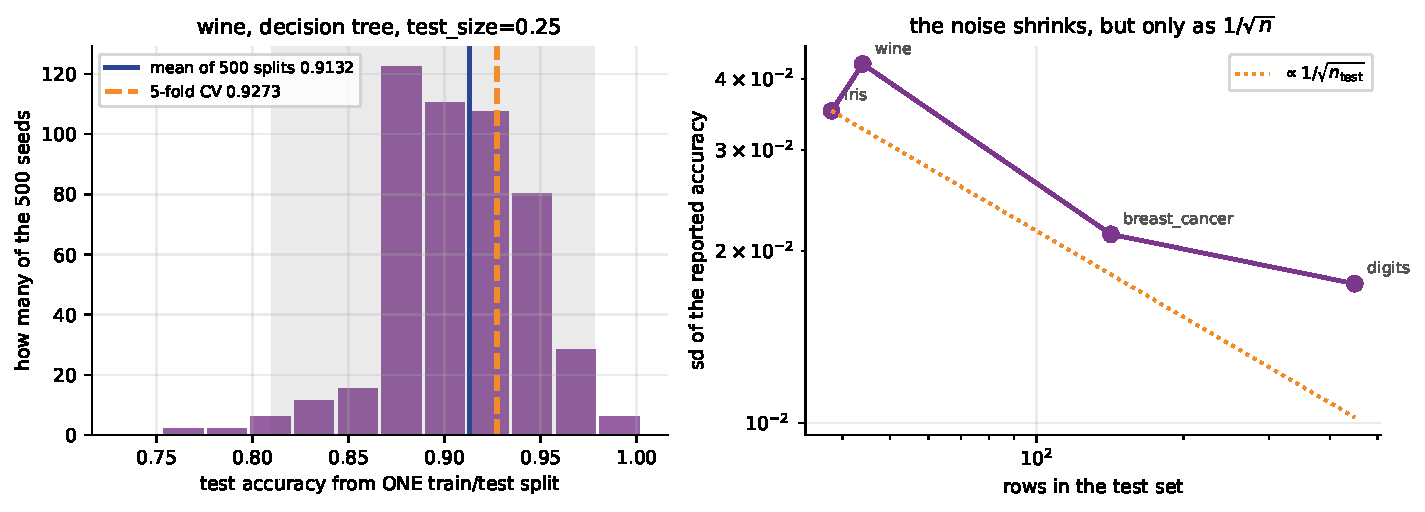
\includegraphics[width=0.90\textwidth]{splitspread.pdf}
  \end{center}
  \begin{center}\small
    Left: the $500$ seeds, with the shaded band the middle $95\%$. Right: the
    same experiment on four datasets. \textbf{More test rows means a tighter
    number --- but only as $1/\sqrt{n}$, so to halve the noise you must
    quadruple the test set}, and every row you move into the test set is a row
    the model cannot learn from.
  \end{center}
\end{frame}

\begin{frame}[fragile,shrink=8]{It is not just noisy --- it ranks models wrongly}
An unpruned tree against a \texttt{max\_depth=3} tree, on the same $500$
splits of wine.
\begin{outblk}
   mean difference -0.0021  sd 0.0276
   the depth-3 tree won on 119 splits, the unpruned tree on 74, tied on 307
   most extreme single-split verdicts: +0.1556 and -0.1333
\end{outblk}
\onslide<2->
\begin{alertblock}{Two models that differ by $0.002$; one experiment that
  swings by $0.29$}
  \footnotesize On average these models are indistinguishable. Yet a single
  split declares a winner $193$ times out of $500$, and the size of its
  verdict runs from $+0.16$ to $-0.13$. \textbf{If your model comparison rests
  on one split, you have measured the split, not the models.}
\end{alertblock}
\onslide<3->
\begin{center}\small
  The fix is not a better seed. It is to \textbf{average over many splits} ---
  which is cross-validation, and it is the middle third of this lecture.
\end{center}
\end{frame}

% =====================================================================
\section[Strategies]{Split strategies: stratified, grouped, ordered}
\label{sec:strategy}

\begin{frame}[shrink=6]{The assumption every random split makes}
  \begin{exampleblock}{}
    \centering
    Rows are \textbf{independent draws from one population}, so any random
    subset is as good as any other.
  \end{exampleblock}
  \vspace{0.3em}
  \begin{center}\small
  \begin{tabular}{@{}lp{4.3cm}p{4.3cm}@{}}
    \toprule
    \textbf{When it fails} & \textbf{Why} & \textbf{What to use}\\
    \midrule
    Skewed classes & a fold may contain few or no minority rows &
      \texttt{StratifiedKFold}, \texttt{stratify=y}\\[4pt]
    Repeated measurements & rows from the same patient, sensor, image or
      customer are near-duplicates & \texttt{GroupKFold},
      \texttt{GroupShuffleSplit}\\[4pt]
    Time order & tomorrow is predicted from yesterday, not from next week &
      \texttt{TimeSeriesSplit}\\
    \bottomrule
  \end{tabular}
  \end{center}
  \begin{block}{The test for all three}
    \small \textbf{Could a test row have been produced by something the
    training set already contains?} If yes, your score is measuring
    recall of the training set.
  \end{block}
\end{frame}

\begin{frame}[fragile,shrink=8]{By hand, then in code: three folds of twelve rows}
The same twelve patients, $9$ healthy and $3$ ill, split three ways.
\begin{outblk}
   KFold(3, shuffle=False)
      fold 1  test rows [0, 1, 2, 3]    y [0, 0, 0, 0]  minority 0
      fold 2  test rows [4, 5, 6, 7]    y [0, 0, 0, 0]  minority 0
      fold 3  test rows [8, 9, 10, 11]  y [0, 1, 1, 1]  minority 3
   StratifiedKFold(3)
      fold 1  test rows [0, 1, 2, 9]    y [0, 0, 0, 1]  minority 1
      fold 2  test rows [3, 4, 5, 10]   y [0, 0, 0, 1]  minority 1
      fold 3  test rows [6, 7, 8, 11]   y [0, 0, 0, 1]  minority 1
\end{outblk}
\onslide<2->
\begin{center}\small
  \textbf{Stratification is not clever. It deals the classes out separately.}
  Three ill patients, three folds, one each --- exactly the arithmetic you did
  on paper. \texttt{KFold} without \texttt{shuffle} takes contiguous blocks,
  which on a sorted file is the worst possible choice.
\end{center}
\end{frame}

\begin{frame}[fragile,shrink=8]{A skewed target, and a fold with nothing to learn from}
$200$ rows, $10$ positives ($5\%$), and the file is sorted by label --- which
is how exports from a database usually arrive.
\begin{outblk}
   KFold(5, shuffle=False)                          positives per fold [10, 0, 0, 0, 0]
   KFold(5, shuffle=True, random_state=0)           positives per fold [3, 1, 2, 3, 1]
   StratifiedKFold(5, shuffle=True, random_state=0) positives per fold [2, 2, 2, 2, 2]
\end{outblk}
\onslide<2->
\begin{outblk}
KFold(5, shuffle=False) class counts, [negatives positives]:
   fold 1  train [160, 0]   test [30, 10]
   fold 2  train [150, 10]  test [40,  0]     ... and the same for folds 3-5
\end{outblk}
\onslide<3->
\begin{alertblock}{Fold 1's training set contains \emph{one class}}
  \footnotesize The classifier cannot be fitted at all, so that fold returns
  \texttt{nan}. Folds $2$--$5$ have no positives to test on, so each scores
  accuracy $1.0000$. \textbf{The reported mean accuracy is $1.0000$ and the
  reported mean recall is $0.0000$.}
\end{alertblock}
\end{frame}

\begin{frame}[shrink=8]{Drawn: stratification on a $5\%$ minority}
  \begin{center}
    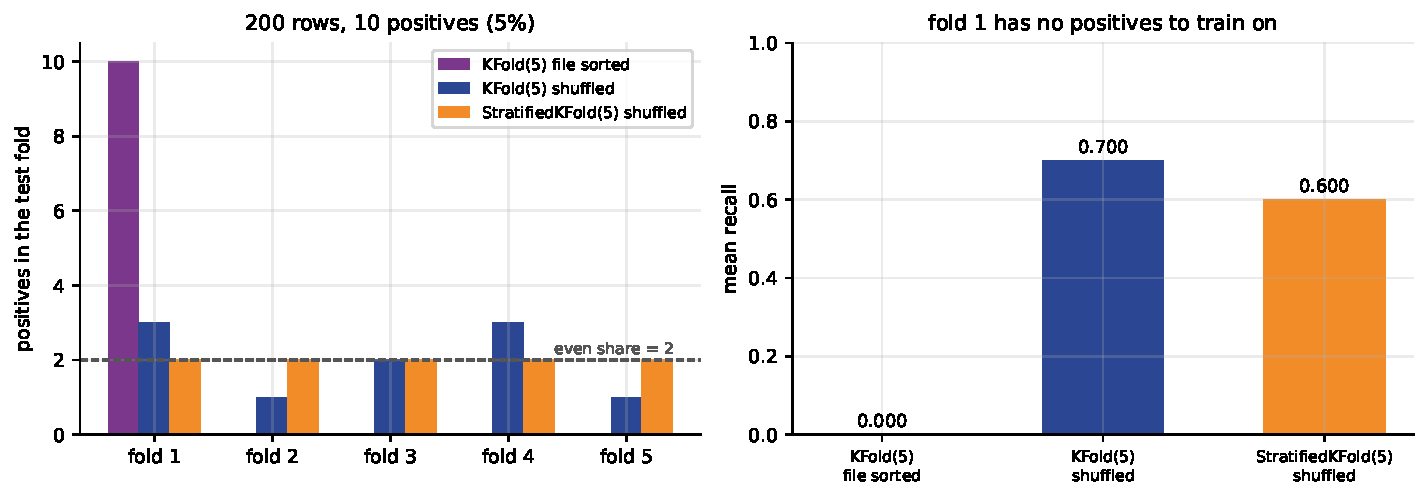
\includegraphics[width=0.88\textwidth]{stratify.pdf}
  \end{center}
  \begin{center}\small
    Left: positives per test fold. Shuffling fixes the catastrophe but still
    leaves folds with $1$ and folds with $3$; stratifying gives $2, 2, 2, 2,
    2$. Right: the recall each choice reports --- $0.000$, $0.700$, $0.600$.
    \textbf{Shuffling alone got a higher number than stratifying, and
    it got it from folds of unequal difficulty.}
  \end{center}
\end{frame}

\begin{frame}[fragile,shrink=8]{Predict first \#2: forty patients, fifteen windows each}
$40$ patients, $15$ signal windows each, $600$ rows. Each patient's
\textbf{diagnosis is a coin flip}. Each patient has a random $10$-dimensional
``fingerprint'' that says nothing about the diagnosis; the features are that
fingerprint plus noise.

\begin{center}
  \textbf{There is nothing to learn. What does a random $5$-fold report?}
\end{center}
\onslide<2->
\begin{outblk}
   random 5-fold, rows shuffled : 1.0000  +/- 0.0000
   GroupKFold(5) by patient     : 0.6483  +/- 0.1984
   overstatement                : +0.3517
   patients in BOTH train and test, random fold 1  : 37 of 40
   patients in BOTH train and test, GroupKFold fold 1: 0
\end{outblk}
\onslide<3->
\begin{alertblock}{$\mathbf{1.0000 \pm 0.0000}$ on a coin flip}
  \footnotesize $37$ of $40$ patients had windows on both sides of fold~1, so
  the model looked up the patient and read off the answer. \textbf{Note the
  second number too: $\pm 0.1984$.} Grouped, the honest estimate has an honest
  error bar, because you have $40$ independent observations and not $600$.
\end{alertblock}
\end{frame}

\begin{frame}[shrink=8]{Drawn: the rows are not independent}
  \begin{center}
    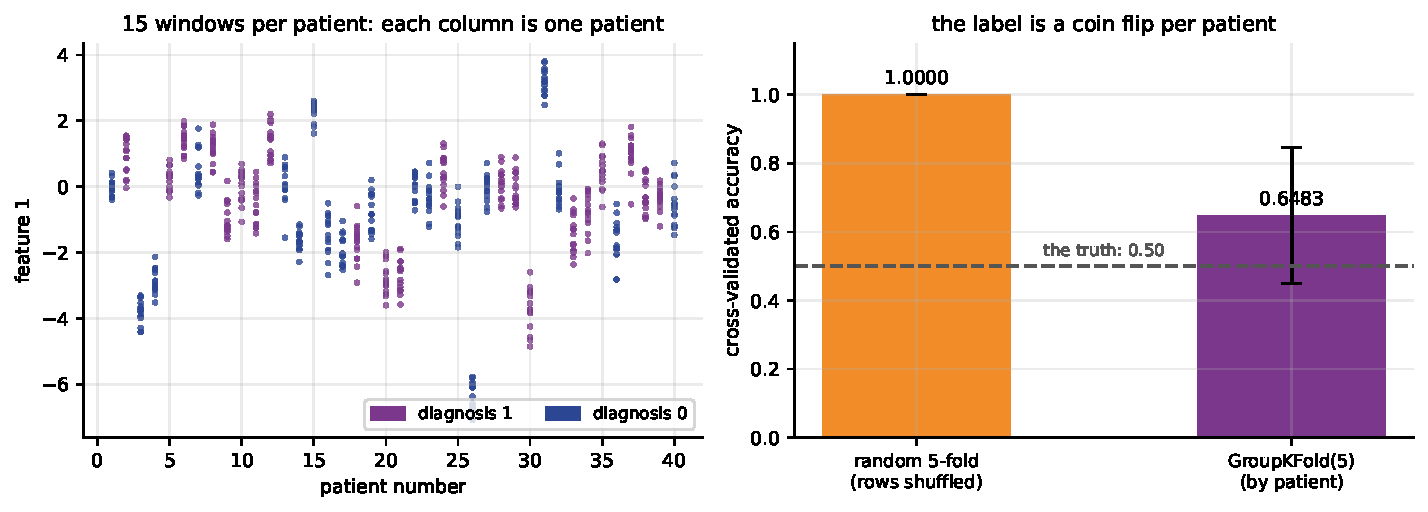
\includegraphics[width=0.88\textwidth]{groups.pdf}
  \end{center}
  \begin{center}\small
    Left: each vertical column is one patient's fifteen windows. They are
    tight, and they all carry the same label. Right: the two verdicts.
    \textbf{Ask ``what is the unit of independence?'' before you split. It is
    the patient, not the window; the customer, not the transaction; the
    document, not the sentence.}
  \end{center}
\end{frame}

\begin{frame}[fragile,shrink=8]{Time-ordered rows: the most persuasive failure in the lecture}
$600$ days of a drifting, seasonal series. Features: the day index and two
seasonal terms. A random forest.
\begin{outblk}
   random 75/25 split               R2 +0.9975
   train on the first 75% of days   R2 -2.7683
   TimeSeriesSplit(5), per fold     [-1.8789, -0.0513, 0.0816, -4.1669, -8.0681]
   TimeSeriesSplit(5), mean         R2 -2.8167
   overstatement from shuffling     +3.8142
   92 of the 150 test days have BOTH neighbours in the training set (61.3%)
\end{outblk}
\onslide<2->
\begin{alertblock}{$R^2 = +0.9975$, and the honest answer is $-2.82$}
  \footnotesize A random split leaves almost every test day \emph{between two
  training days}, so the model interpolates. In production it must
  \textbf{extrapolate}, and a forest cannot: its predictions are bounded by
  the training targets. \textbf{An $R^2$ below zero means you would have done
  better predicting the mean.}
\end{alertblock}
\end{frame}

\begin{frame}[shrink=8]{Drawn: interpolation against extrapolation}
  \begin{center}
    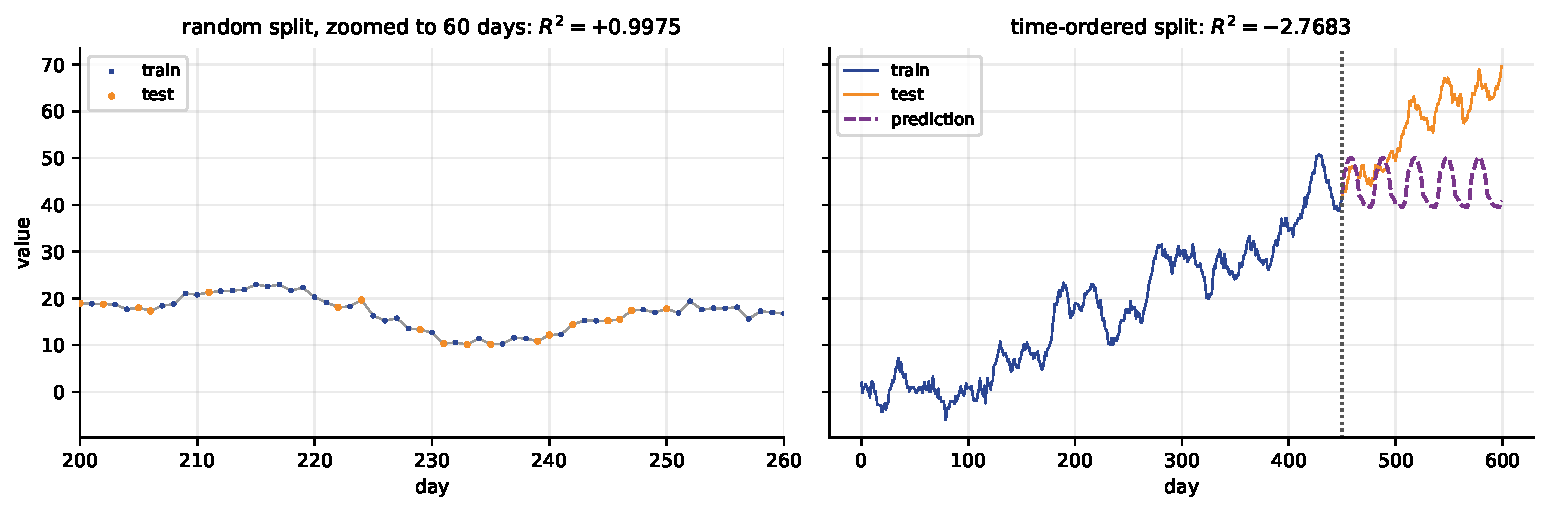
\includegraphics[width=0.90\textwidth]{timeseries.pdf}
  \end{center}
  \begin{center}\small
    Left, zoomed to sixty days: orange test points sitting between blue
    training points. Right: trained on the first $450$ days, the forest's
    prediction \textbf{flattens the moment it leaves the training range} while
    the series keeps climbing.
  \end{center}
\end{frame}

\begin{frame}[fragile,shrink=8]{And the wrong splitter chooses the wrong model}
Two candidates on the same $600$ days.
\begin{outblk}
A: calendar features + random forest   shuffled 5-fold R2 +0.9974
                                       TimeSeriesSplit R2 -2.8167
B: lag-1 + trailing mean + linear      shuffled 5-fold R2 +0.9967
                                       TimeSeriesSplit R2 +0.9230
\end{outblk}
\onslide<2->
\begin{alertblock}{Shuffled cross-validation ranks A above B, and A is useless}
  \footnotesize $0.9974$ against $0.9967$: on the shuffled evidence you ship
  model A. Evaluated in time order, A is $-2.82$ and B is $+0.92$.
  \textbf{The wrong splitter does not merely inflate a number; it inverts the
  decision the number was for.}
\end{alertblock}
\onslide<3->
\begin{center}\small
  Same rule as the grouped case: \textbf{if a test row could not have existed
  at the moment of prediction, it must not be in the test set.}
\end{center}
\end{frame}

\begin{frame}[shrink=8]{Drawn: six splitters, from their actual indices}
  \begin{center}
    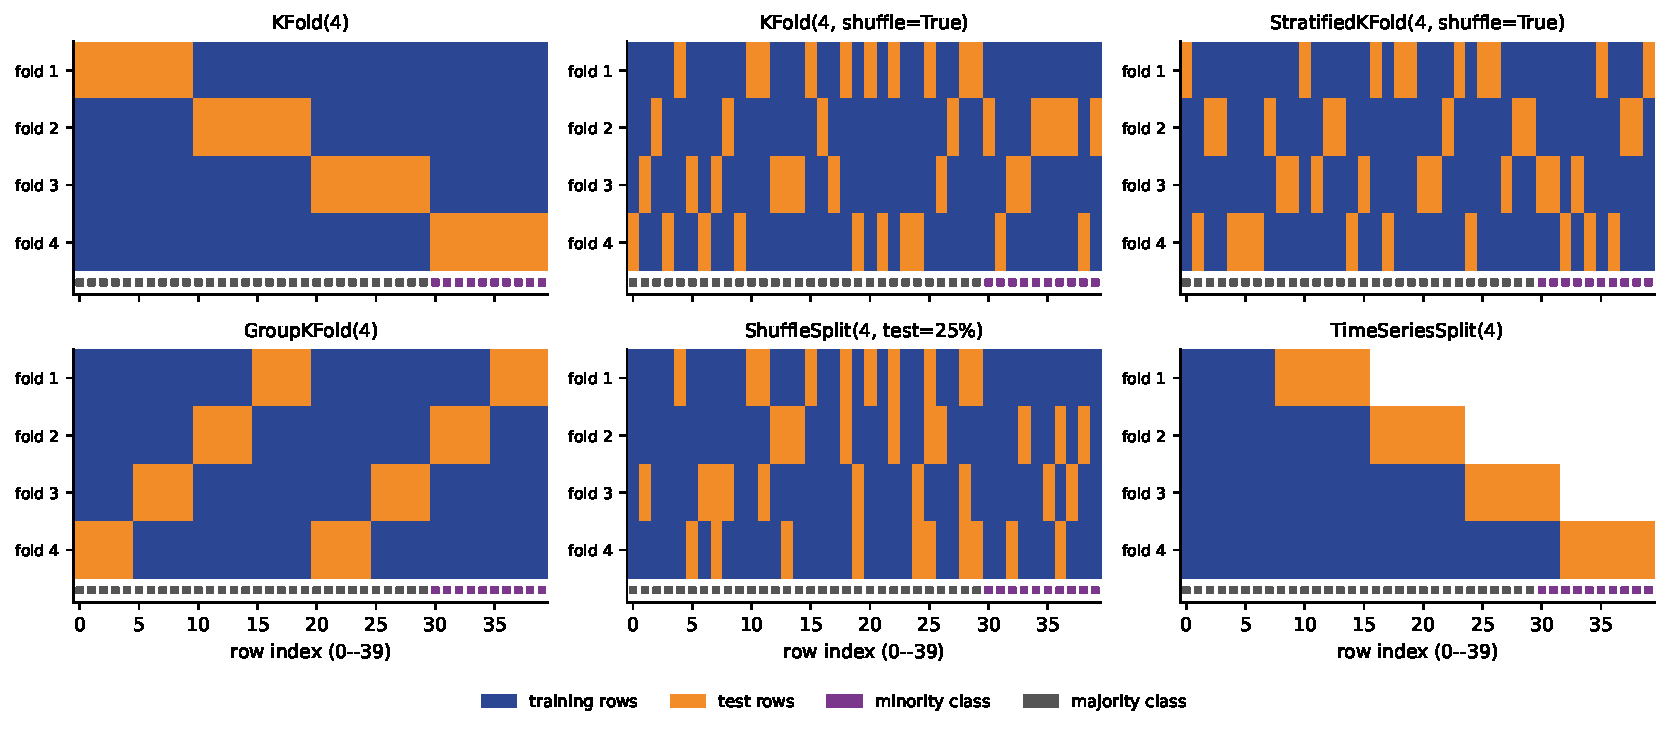
\includegraphics[width=0.93\textwidth]{cvsplits.pdf}
  \end{center}
  \begin{center}\small
    Forty rows, ten of them minority, arriving sorted, in eight groups of
    five. Minority rows per test fold: \texttt{KFold} $[0,0,0,10]$; shuffled
    $[0,6,2,2]$; stratified $[2,2,3,3]$; \texttt{GroupKFold} $[5,5,0,0]$;
    \texttt{TimeSeriesSplit} $[0,0,2,8]$. \textbf{Every picture here was drawn
    from the indices the splitter really returned.}
  \end{center}
\end{frame}

% =====================================================================
\section[Cross-validation]{Cross-validation}
\label{sec:cv}

\begin{frame}[shrink=6]{$k$-fold: use every row for testing, exactly once}
  \begin{columns}[T]
    \begin{column}{0.5\textwidth}
      \begin{block}{The recipe}
        \begin{enumerate}\small
          \item Cut the rows into $k$ folds.
          \item For each fold: train on the other $k-1$, test on this one.
          \item Report the mean of the $k$ scores --- and the spread.
        \end{enumerate}
      \end{block}
      \begin{exampleblock}{What it buys}
        \small Every row is tested on once, so the estimate uses all $n$ rows
        rather than $n/4$; and you get $k$ numbers instead of one, so you can
        see how variable the answer is.
      \end{exampleblock}
    \end{column}
    \begin{column}{0.47\textwidth}
      \begin{block}{The arithmetic, by hand}
        \small With $n = 5000$ rows:
        \begin{center}\scriptsize
        \begin{tabular}{@{}lrrr@{}}
          \toprule
          & fits & rows each & row-fits\\
          \midrule
          $2$-fold & $2$ & $2500$ & $5{,}000$\\
          $5$-fold & $5$ & $4000$ & $20{,}000$\\
          $10$-fold & $10$ & $4500$ & $45{,}000$\\
          LOOCV & $5000$ & $4999$ & $24{,}995{,}000$\\
          \bottomrule
        \end{tabular}
        \end{center}
        \small \textbf{$k$-fold costs $k$ times a single fit. That is the
        whole cost model.}
      \end{block}
    \end{column}
  \end{columns}
\end{frame}

\begin{frame}[fragile,shrink=8]{$k$, measured: bias, and cost}
\texttt{load\_breast\_cancer}, $569$ rows, \texttt{StandardScaler} $+$
logistic regression.
\begin{outblk}
   2-fold      2 fits   trains on 284 rows   accuracy 0.9859     0.01 s
   5-fold      5 fits   trains on 455 rows   accuracy 0.9789     0.01 s
   10-fold    10 fits   trains on 512 rows   accuracy 0.9772     0.03 s
   20-fold    20 fits   trains on 540 rows   accuracy 0.9790     0.06 s
   LOOCV     569 fits   trains on 568 rows   accuracy 0.9789     1.62 s
   LOOCV: 569 fits against 5-fold's 5 = 113.8x as many (the seconds vary)
\end{outblk}
\onslide<2->
\begin{alertblock}{Read the second column, not the third}
  \footnotesize $2$-fold trains on $284$ rows and $20$-fold on $540$.
  \textbf{Small $k$ is pessimistic because it starves the model} --- which is
  the bias of $k$-fold, and here it is worth about $0.002$ because a
  $569$-row learning curve is already flat. On a small or steep dataset it is
  worth much more.
\end{alertblock}
\onslide<3->
\begin{center}\small
  Measured learning curve: $50$ rows $\to 0.9566$, $200 \to 0.9709$,
  $540 \to 0.9776$.
\end{center}
\end{frame}

\begin{frame}[fragile,shrink=8]{Predict first \#3: which $k$ gives the steadiest answer?}
Repeat the whole cross-validation with $40$ different shuffles and look at the
spread of \textbf{the mean}.

\begin{center}
  \textbf{Textbooks say LOOCV has high variance. Does it, here?}
\end{center}
\onslide<2->
\begin{outblk}
    2-fold   mean of means 0.9754   sd of the mean 0.0042   range 0.0194
    5-fold   mean of means 0.9782   sd of the mean 0.0030   range 0.0123
   10-fold   mean of means 0.9786   sd of the mean 0.0025   range 0.0106
   20-fold   mean of means 0.9791   sd of the mean 0.0019   range 0.0072
   LOOCV     mean          0.9789   sd of the mean 0.0000   (deterministic)
   one 80/20 split, 40 seeds: mean 0.9772  sd 0.0114  range 0.0526
\end{outblk}
\onslide<3->
\begin{alertblock}{On this dataset the variance \emph{falls} with $k$, and
  LOOCV has none}
  \footnotesize LOOCV does not shuffle, so re-running it changes nothing.
  \textbf{Report the experiment you ran, not the one the textbook predicts:}
  the high-variance claim for LOOCV is about \emph{correlated folds} across
  \emph{different datasets}, and it is not what this measurement shows. What
  LOOCV certainly is, is expensive: $569$ fits against $5$-fold's $5$,
  $113.8\times$ as many on any machine. Quote that, not the seconds --- the
  wall-clock ratio wandered between $112$ and $131$ over four repeats of the
  same measurement.
\end{alertblock}
\end{frame}

\begin{frame}[fragile,shrink=8]{Two traps in that table}
\begin{outblk}
   sd ACROSS FOLDS: 5-fold 0.0142   LOOCV 0.1437   <- not comparable
\end{outblk}
\onslide<2->
\begin{columns}[T]
  \begin{column}{0.5\textwidth}
    \begin{alertblock}{$0.1437$ is not ``LOOCV is unstable''}
      \small Each LOOCV fold scores $0$ or $1$ on a single row, so the
      across-fold sd is just $\sqrt{p(1-p)}$. \textbf{It says nothing about
      the estimator.} The number that matters is the sd of the \emph{mean},
      and that is the previous slide.
    \end{alertblock}
  \end{column}
  \begin{column}{0.47\textwidth}
    \begin{block}{And a single split is worse than all of them}
      \small One $80/20$ split: sd $0.0114$, range $0.0526$. Five-fold:
      sd $0.0030$. \textbf{Cross-validating is roughly four times steadier
      here, for five times the compute.}
    \end{block}
  \end{column}
\end{columns}
\end{frame}

\begin{frame}[shrink=8]{Drawn: bias, variance and cost against $k$}
  \begin{center}
    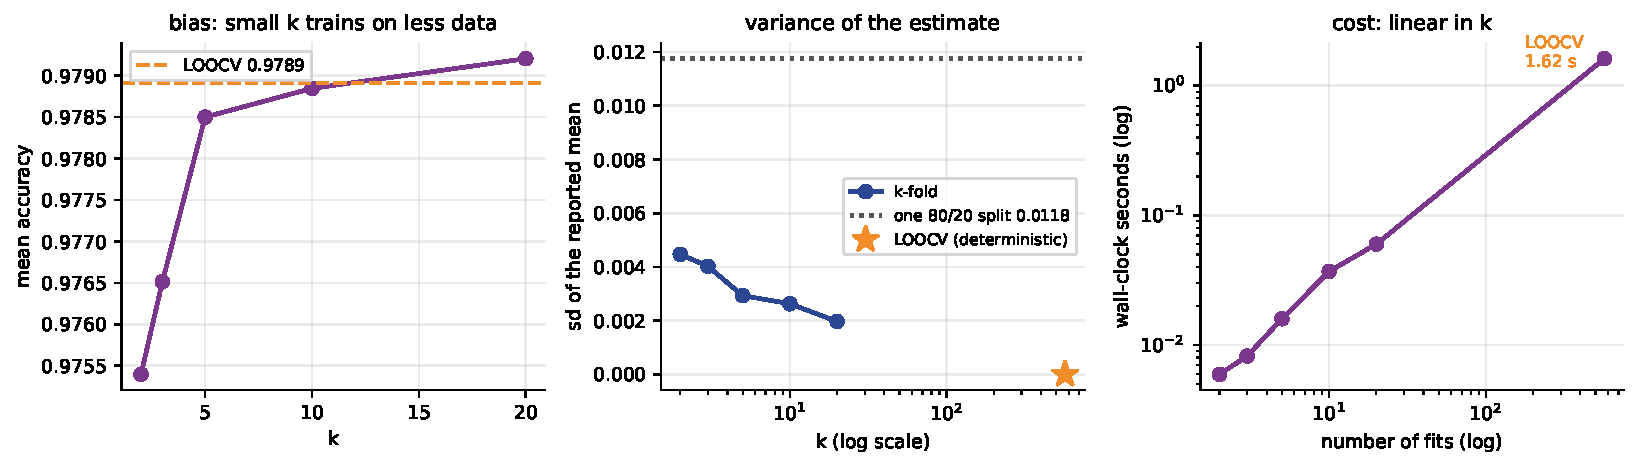
\includegraphics[width=0.94\textwidth]{kchoice.pdf}
  \end{center}
  \begin{center}\small
    Left: the mean rises with $k$ and flattens --- that is the bias going
    away. Middle: the spread of the estimate falls with $k$; the dotted line
    is a single $80/20$ split. Right: cost is exactly linear in the number of
    fits. \textbf{Five or ten folds is where these three curves meet.}
  \end{center}
\end{frame}

\begin{frame}[fragile,shrink=8]{More folds, or more repeats?}
\begin{outblk}
   StratifiedKFold(5)                    5 fits  accuracy 0.9789 +/- 0.0142   0.02 s
   RepeatedStratifiedKFold(5 x 10)      50 fits  accuracy 0.9772 +/- 0.0147   0.17 s
   StratifiedShuffleSplit(50, test 20%) 50 fits  accuracy 0.9767 +/- 0.0122   0.18 s
\end{outblk}
\onslide<2->
\begin{center}\small
  \begin{tabular}{@{}lp{7.6cm}@{}}
    \toprule
    \texttt{StratifiedKFold(5)} & the default. Use it.\\
    \texttt{RepeatedStratifiedKFold} & when $n$ is small and you need the
      estimate to stop wobbling.\\
    \texttt{ShuffleSplit} & when you want the test size and the number of
      repeats to be independent of each other.\\
    \texttt{LeaveOneOut} & when $n$ is tiny and a fit is cheap.\\
    \texttt{GroupKFold} / \texttt{TimeSeriesSplit} & whenever the rows are not
      independent. \textbf{Not optional.}\\
    \bottomrule
  \end{tabular}
\end{center}
\onslide<3->
\begin{center}\small
  \textbf{Repeating is cheaper than it looks and it is the honest way to say
  ``this difference is real''.}
\end{center}
\end{frame}

% =====================================================================
\section[Tuning]{Tuning honestly: validation sets and nested CV}
\label{sec:nested}

\begin{frame}[fragile,shrink=8]{The moment you tune, the score stops being an estimate}
Three-way split on breast\_cancer: train $341$, validation $114$, test $114$.
\begin{outblk}
      C=  0.01  validation 0.9561
      C=  0.10  validation 0.9561
      C=  1.00  validation 0.9474
      C= 10.00  validation 0.9474
      C=100.00  validation 0.9298
   chosen C=0.01   validation 0.9561   TEST 0.9386
\end{outblk}
\onslide<2->
\begin{alertblock}{$0.9561$ is a \emph{maximum over five tries}; $0.9386$ is
  the estimate}
  \footnotesize You picked the largest of five noisy numbers, so it is biased
  upward by construction --- the same reason the tallest of five random
  people is taller than average. \textbf{The test set is the only number in
  that block you may quote}, and you may quote it once.
\end{alertblock}
\onslide<3->
\begin{center}\small
  Cross-validation replaces the validation \emph{set}; it does not remove the
  need for a validation \emph{step}. If the tuning happens inside the same
  folds you report, the bias comes straight back.
\end{center}
\end{frame}

\begin{frame}[fragile,shrink=8]{Predict first \#4: tuning on pure noise}
$100$ rows, $200$ features, everything from $\mathcal{N}(0,1)$. The labels are
\textbf{coin flips}. Tune an RBF SVM over $5$ values of $C$ and $4$ of
$\gamma$ with $5$-fold cross-validation, then report the best cross-validated
score the search found.

\begin{center}
  \textbf{The truth is $0.50$. What comes out?}
\end{center}
\onslide<2->
\begin{outblk}
   tune and report on the SAME folds : 0.5820  +/- 0.0314
   nested cross-validation           : 0.5265  +/- 0.0419
   optimism                          : +0.0555
   the wrong way beat 0.5 on 20 of 20 trials
\end{outblk}
\onslide<3->
\begin{alertblock}{$+0.0555$ out of thin air, on $20$ trials out of $20$}
  \footnotesize \texttt{best\_score\_} is the \textbf{maximum} of twenty
  cross-validated numbers, each with a standard error of a few points. The
  maximum of twenty noisy numbers is bigger than their mean.
  \textbf{\texttt{best\_score\_} is a selection, not an estimate, and it must
  never be reported as performance.}
\end{alertblock}
\end{frame}

\begin{frame}[fragile,shrink=8]{And on real data, where there is signal}
A $120$-row subsample of breast\_cancer, the same grid, $20$ trials.
\begin{outblk}
   tune and report on the SAME folds : 0.9529  +/- 0.0054
   nested cross-validation           : 0.9317  +/- 0.0094
   optimism                          : +0.0212
   paired t over 20 trials: t = 9.58, p = 1.1e-08
   the wrong way was higher on 19 of 20 trials
\end{outblk}
\onslide<2->
\begin{outblk}
grid size drives it (pure noise, every row should read 0.5000):
    1 combinations   same-fold 0.5467   nested 0.5467   optimism +0.0000
    4 combinations   same-fold 0.5767   nested 0.5567   optimism +0.0200
   20 combinations   same-fold 0.5833   nested 0.5217   optimism +0.0617
   60 combinations   same-fold 0.5850   nested 0.5067   optimism +0.0783
\end{outblk}
\onslide<3->
\begin{alertblock}{With one combination the optimism is \emph{exactly} zero}
  \footnotesize That row is the proof of the mechanism: with nothing to
  choose between, there is nothing to over-fit. \textbf{The optimism is the
  price of the search, and it grows with the size of the grid.}
\end{alertblock}
\end{frame}

\begin{frame}[shrink=8]{Drawn: twenty trials, paired}
  \begin{center}
    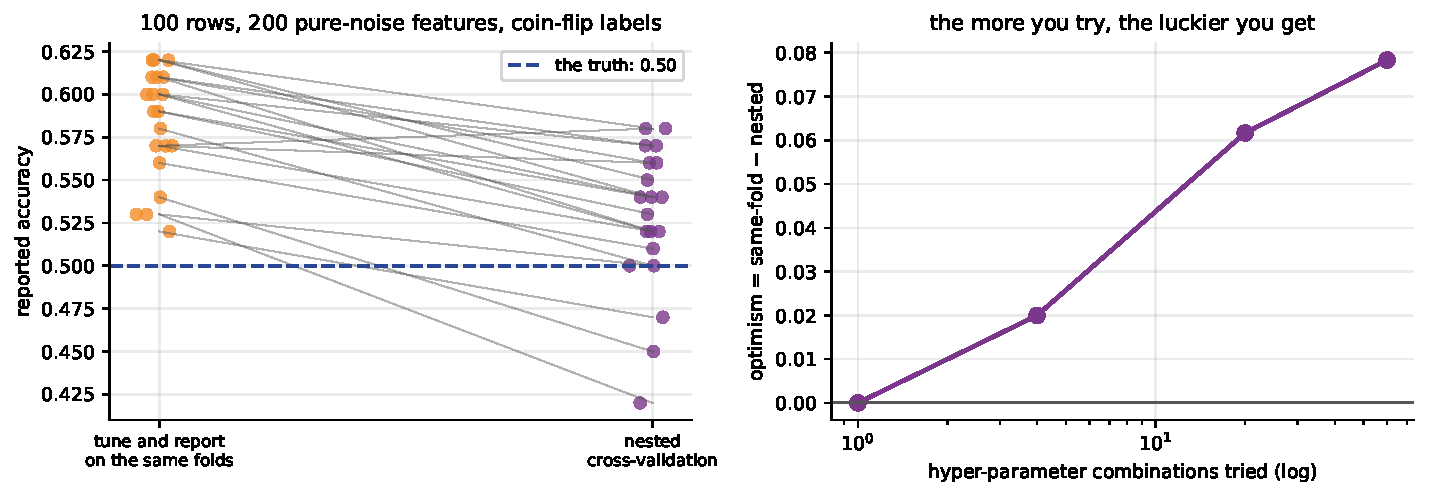
\includegraphics[width=0.90\textwidth]{nested.pdf}
  \end{center}
  \begin{center}\small
    Left: each grey line is one trial. Every orange point is above $0.50$;
    the purple points scatter around it as they should. Right: optimism
    against grid size, from $+0.0000$ at one combination to $+0.0783$ at
    sixty.
  \end{center}
\end{frame}

\begin{frame}[fragile,shrink=6]{Nested cross-validation, in four lines}
\begin{lstlisting}
inner = StratifiedKFold(5, shuffle=True, random_state=0)
outer = StratifiedKFold(5, shuffle=True, random_state=0)
search = GridSearchCV(pipe, grid, cv=inner)     # chooses the hyper-parameters
score  = cross_val_score(search, X, y, cv=outer)  # estimates the performance
\end{lstlisting}
\begin{center}\small
  The inner loop \textbf{selects}; the outer loop \textbf{estimates}. The
  outer test fold is never involved in choosing anything --- not the scaler's
  mean, not the feature subset, not $C$, not $\gamma$.
\end{center}
\onslide<2->
\begin{alertblock}{Cost, and the honest answer to ``is it worth it?''}
  \footnotesize $5 \times 5 \times 20 = 500$ fits instead of $100$.
  \textbf{Use nested CV when you are reporting a number. Use plain
  \texttt{GridSearchCV} when you are choosing a model and will evaluate it
  later on a held-out test set.} Both are correct; quoting
  \texttt{best\_score\_} as your result is not.
\end{alertblock}
\end{frame}

% =====================================================================
\section[Imbalance]{Imbalanced data}
\label{sec:imbal}

\begin{frame}[shrink=8]{By hand: one thousand patients, ten of them ill}
  A model that always says ``healthy'':
  \begin{center}\small
  \begin{tabular}{@{}lcc@{}}
    \toprule
    & predicted healthy & predicted ill\\
    \midrule
    actually healthy & $\mathrm{TN} = 990$ & $\mathrm{FP} = 0$\\
    actually ill     & $\mathrm{FN} = 10$  & $\mathrm{TP} = 0$\\
    \bottomrule
  \end{tabular}
  \end{center}
  \[
    \text{accuracy} = \frac{990 + 0}{1000} = \mathbf{0.990},
    \qquad
    \text{recall} = \frac{0}{0 + 10} = \mathbf{0}, \qquad
    \text{precision} = \frac{0}{0} \ \text{undefined}.
  \]
  \begin{alertblock}{$99\%$ accurate, and it has never once found an ill patient}
    \small Accuracy is $\frac{\mathrm{TP}+\mathrm{TN}}
    {\mathrm{TP}+\mathrm{TN}+\mathrm{FP}+\mathrm{FN}}$, and when
    $\mathrm{TN}$ is $99\%$ of the table, accuracy is a report on
    $\mathrm{TN}$. \textbf{Recall asks about the row you care about;
    precision asks about the column you act on.}
  \end{alertblock}
\end{frame}

\begin{frame}[fragile,shrink=8]{Predict first \#5}
$5000$ rows, $50$ positives ($1\%$), twenty features, six of them
informative. First a \texttt{DummyClassifier} that always predicts the
majority; then a real logistic regression.

\begin{center}
  \textbf{Which of the two has the higher accuracy?}
\end{center}
\onslide<2->
\begin{outblk}
   DummyClassifier(most_frequent)  accuracy 0.9900  recall 0.0000  PR-AUC 0.0100
   LogisticRegression              accuracy 0.9867  recall 0.0000  PR-AUC 0.1075
      confusion matrix [[1480, 5], [15, 0]]     ROC-AUC 0.8553
   accuracy says the model is worth -0.0033 over the dummy
   PR-AUC says it is worth        +0.0975
\end{outblk}
\onslide<3->
\begin{alertblock}{The dummy \emph{wins} on accuracy}
  \footnotesize The real model has learned a great deal --- ROC-AUC $0.8553$,
  PR-AUC nearly eleven times chance --- and at the default threshold of
  $0.5$ it still labels almost everything negative, so accuracy \emph{rates
  it below a model that has learned nothing.} \textbf{Two failures at once:
  the metric is wrong, and the threshold is wrong.}
\end{alertblock}
\end{frame}

\begin{frame}[shrink=8]{Drawn: five metrics, three models}
  \begin{center}
    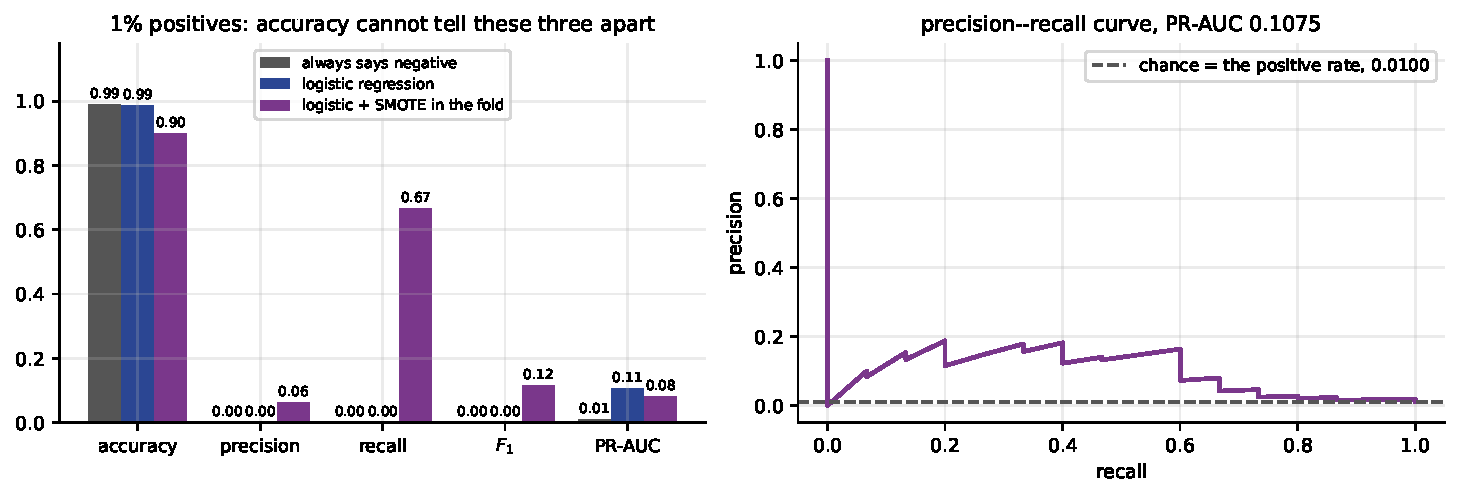
\includegraphics[width=0.90\textwidth]{imbalance.pdf}
  \end{center}
  \begin{center}\small
    Left: accuracy is $0.99, 0.99, 0.90$ for a useless model, a good model and
    a good model with the threshold moved. \textbf{The one metric that is the
    same for all three is the one everybody quotes.} Right: the
    precision--recall curve, whose baseline is the positive rate $0.01$, not
    $0.5$.
  \end{center}
\end{frame}

\begin{frame}[shrink=6]{Four things you can do about it}
  \begin{center}\small
  \begin{tabular}{@{}lp{4.5cm}p{4.3cm}@{}}
    \toprule
    & \textbf{What it does} & \textbf{What it costs}\\
    \midrule
    \textbf{Random oversampling} & copies minority rows until the classes
      balance & duplicates: the model can memorise them\\[4pt]
    \textbf{Random undersampling} & throws majority rows away until the
      classes balance & discards most of your data\\[4pt]
    \textbf{SMOTE} & invents minority rows between existing ones &
      interpolates into regions where no data was observed\\[4pt]
    \textbf{Class weights} & multiplies the loss of minority errors, no rows
      added or removed & none, and it is one keyword argument\\
    \bottomrule
  \end{tabular}
  \end{center}
  \begin{alertblock}{And the one that is not on the list}
    \small \textbf{Move the threshold.} A classifier gives you a probability;
    $0.5$ is a convention, not a result. Choosing the threshold from the
    precision--recall curve costs nothing and is often all you need.
  \end{alertblock}
\end{frame}

\begin{frame}[fragile,shrink=8]{By hand: SMOTE is one line of arithmetic}
Two minority patients, $A = (1, 1)$ and $B = (3, 5)$. SMOTE draws
$u \sim \mathcal{U}(0,1)$ and returns $A + u(B - A)$:
\begin{outblk}
   u = 0.00  ->  [1.0, 1.0]      (that is A)
   u = 0.25  ->  [1.5, 2.0]
   u = 0.50  ->  [2.0, 3.0]      (the midpoint)
   u = 1.00  ->  [3.0, 5.0]      (that is B)
\end{outblk}
\onslide<2->
\begin{lstlisting}
nn = NearestNeighbors(n_neighbors=6).fit(Xmin)   # k = 5 minority neighbours
_, ind = nn.kneighbors(Xmin);  ind = ind[:, 1:]  # drop the point itself
new = Xmin[base] + u * (Xmin[nbr] - Xmin[base])  # a point on the segment
\end{lstlisting}
\onslide<3->
\begin{center}\small
  That is the whole of Chawla et al.\ (2002). \textbf{It is not generating
  data; it is asserting that the straight line between two ill patients is
  full of ill patients.} Sometimes true. Sometimes exactly wrong.
\end{center}
\end{frame}

\begin{frame}[fragile,shrink=8]{The three resamplers, on the $1\%$ problem}
\begin{outblk}
   random oversample   train  3500 ->  6930 rows,  class counts [3465, 3465]
   random undersample  train  3500 ->    70 rows,  class counts [35, 35]
   SMOTE               train  3500 ->  6930 rows,  class counts [3465, 3465]
      3430 of the 3465 minority rows are synthetic (99.0%)
      distinct minority rows: SMOTE 3465, oversampling 35
\end{outblk}
\onslide<2->
\begin{alertblock}{Read the last line twice}
  \footnotesize Oversampling turns $35$ patients into $3465$ rows that are
  copies of \textbf{$35$ distinct patients}. SMOTE turns them into $3465$
  distinct points --- but every one of them lies on a segment between two of
  the same $35$. \textbf{Neither method has added a single new observation.}
\end{alertblock}
\onslide<3->
\begin{center}\small
  And undersampling kept $70$ of $3500$ rows: \textbf{$99.0\%$ of the
  negatives were thrown away.}
\end{center}
\end{frame}

\begin{frame}[shrink=8]{Drawn: what each resampler does to the picture}
  \begin{center}
    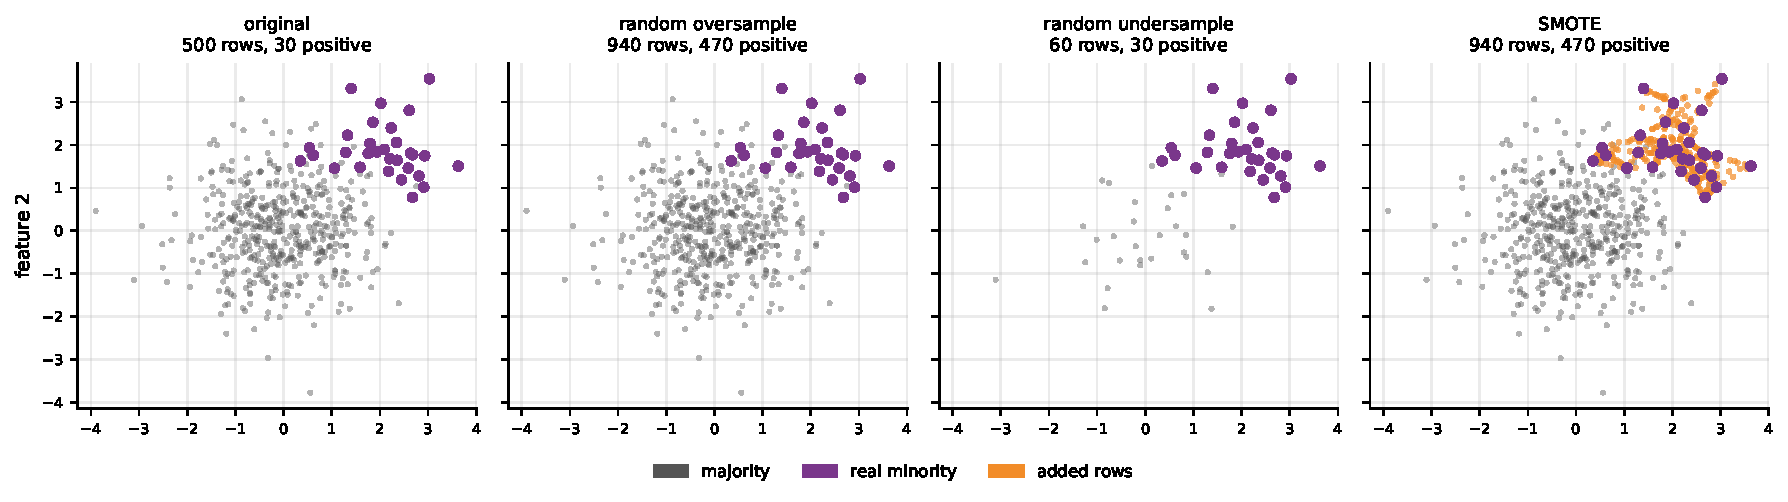
\includegraphics[width=0.98\textwidth]{resample.pdf}
  \end{center}
  \begin{center}\small
    Purple is real minority, orange is added. Oversampling adds nothing you
    can see --- the new points are \emph{on top of} the old ones. SMOTE's
    additions trace the segments between neighbours, which is why the cloud
    looks like a web. Undersampling simply deletes most of the grey.
  \end{center}
\end{frame}

\begin{frame}[fragile,shrink=8]{Does any of it help? Measure, and report what you find}
Five-fold, resampled \textbf{inside} each fold, logistic regression.
\begin{outblk}
   method                 accuracy precision  recall      F1   PR-AUC
   always negative         0.9900    0.0000  0.0000  0.0000   0.0100
   no treatment            0.9890    0.1333  0.0400  0.0583   0.1916
   random oversample       0.8542    0.0517  0.7800  0.0969   0.1369
   random undersample      0.7944    0.0390  0.8200  0.0744   0.1142
   SMOTE                   0.8814    0.0612  0.7600  0.1133   0.1404
   class_weight balanced   0.8556    0.0520  0.7800  0.0974   0.1368
\end{outblk}
\onslide<2->
\begin{alertblock}{Recall $0.04 \rightarrow 0.78$; PR-AUC $0.19 \rightarrow 0.14$}
  \footnotesize Every treatment transforms recall and none of them improves
  the \emph{ranking}: PR-AUC is highest with no treatment at all.
  \textbf{Resampling moves the decision threshold. It does not create
  information.} That is a genuine result and it should be reported, not
  hidden.
\end{alertblock}
\onslide<3->
\begin{center}\small
  Note also that \texttt{class\_weight="balanced"} matches random
  oversampling to three decimal places --- as it should, since weighting a row
  by $w$ and copying it $w$ times are the same thing to the loss function.
\end{center}
\end{frame}

\begin{frame}[fragile,shrink=8]{Predict first \#6: one line in the wrong place}
The same SMOTE, the same model, the same five folds. The only difference:
\texttt{X, y = smote(X, y)} is called \emph{before} \texttt{cross\_val\_score}
instead of inside the loop.

\begin{center}
  \textbf{How much does that move $F_1$?}
\end{center}
\onslide<2->
\begin{outblk}
   random oversample  BEFORE the split : F1 0.8607  recall 0.8655  PR-AUC 0.9176
   random oversample  INSIDE each fold : F1 0.0969  recall 0.7800  PR-AUC 0.1369
   SMOTE              BEFORE the split : F1 0.8942  recall 0.9067  PR-AUC 0.9207
   SMOTE              INSIDE each fold : F1 0.1133  recall 0.7600  PR-AUC 0.1404
   overstatement in F1: +0.7638 (oversample)   +0.7809 (SMOTE)
\end{outblk}
\onslide<3->
\begin{alertblock}{$\mathbf{0.894}$ against $\mathbf{0.113}$}
  \footnotesize An eight-fold overstatement, from moving one line. This is by
  a wide margin the most common mistake in student projects on imbalanced
  data, and it produces exactly the sort of number that makes a report look
  finished.
\end{alertblock}
\end{frame}

\begin{frame}[fragile,shrink=8]{Why: the same row is on both sides}
\begin{outblk}
   after oversampling before the split, fold 1 has 1980 test rows
   of which 990 (50.0%) are byte-identical to a training row
   among the 990 MINORITY test rows, 990 (100.0%) are copies
\end{outblk}
\onslide<2->
\begin{center}\small
  \textbf{Every single minority row in the test fold is a copy of a row the
  model trained on.} The model is not being tested; it is being asked to
  remember. SMOTE is only slightly less blatant: its synthetic points are
  built \emph{from} the training points, so they carry the same information
  across the boundary.
\end{center}
\onslide<3->
\begin{alertblock}{The rule, stated once}
  \footnotesize \textbf{Resampling is part of the model, so it happens inside
  the fold, on the training part only. The test fold keeps its natural class
  balance --- because that is the balance you will meet in production.}
\end{alertblock}
\end{frame}

\begin{frame}[shrink=8]{Drawn: the same code, one line moved}
  \begin{center}
    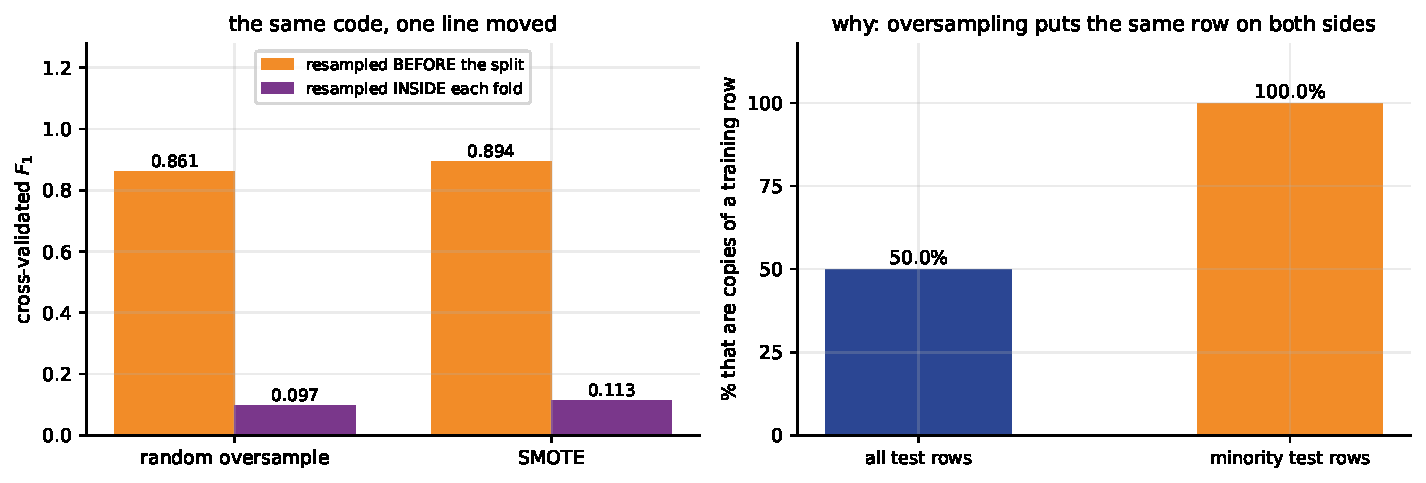
\includegraphics[width=0.90\textwidth]{resampleleak.pdf}
  \end{center}
  \begin{center}\small
    Left: $F_1$ for both resamplers, before and inside. Right: the mechanism
    --- half of every test fold, and \textbf{all} of its minority half, are
    duplicates of training rows.
  \end{center}
\end{frame}

\begin{frame}[fragile,shrink=8]{How bad does imbalance have to get?}
The same generator, the minority fraction swept from $50\%$ to $0.2\%$.
\begin{outblk}
   minority  50.0% (2500 rows)  always-negative 0.5000  accuracy 0.8586  recall 0.8704  PR-AUC 0.9063
   minority  20.0% (1000 rows)  always-negative 0.8000  accuracy 0.8874  recall 0.6210  PR-AUC 0.7532
   minority  10.0% ( 500 rows)  always-negative 0.9000  accuracy 0.9260  recall 0.4400  PR-AUC 0.6098
   minority   5.0% ( 250 rows)  always-negative 0.9500  accuracy 0.9544  recall 0.2720  PR-AUC 0.4392
   minority   1.0% (  50 rows)  always-negative 0.9900  accuracy 0.9890  recall 0.0400  PR-AUC 0.1916
   minority   0.2% (  10 rows)  always-negative 0.9980  accuracy 0.9980  recall 0.0000  PR-AUC 0.0277
\end{outblk}
\onslide<2->
\begin{alertblock}{Two columns moving in opposite directions}
  \footnotesize As the problem gets harder, \textbf{accuracy goes up} ---
  $0.86$ at balance, $0.998$ at $0.2\%$ --- while recall falls to zero.
  \textbf{Reported accuracy is a measure of how imbalanced your data is.}
  There is no threshold at which imbalance ``starts''; it is a slope.
\end{alertblock}
\end{frame}

\begin{frame}[fragile,shrink=6]{The whole thing in one place}
\begin{lstlisting}
rng = np.random.default_rng(0)              # the one seed for this lecture
Xtr, Xte, ytr, yte = train_test_split(X, y, test_size=0.3, stratify=y,
                                      random_state=0)
for C in grid:                              # tune on the TRAINING part only
    for tr, va in StratifiedKFold(5, shuffle=True,
                                  random_state=0).split(Xtr, ytr):
        Xa, ya = smote(Xtr[tr], ytr[tr], rng)   # resample INSIDE the fold
        ...score on Xtr[va], which was never resampled...
final = fit(smote(Xtr, ytr, rng), best_C)   # refit on all the training rows
report(final, Xte, yte)                     # the test set, once
\end{lstlisting}
\begin{outblk}
   chosen C=0.01 (inner F1 0.1271)
   held-out TEST: accuracy 0.8940  precision 0.0610  recall 0.6667  F1 0.1117  PR-AUC 0.0842
   confusion matrix [[1331, 154], [5, 10]]
\end{outblk}
\onslide<2->
\begin{center}\small
  \textbf{Ten of the fifteen ill patients found, at the cost of $154$ false
  alarms.} That is the real trade-off, stated in patients rather than in
  decimals --- and it is a clinical decision, not a modelling one.
\end{center}
\end{frame}

% =====================================================================
\section{Summary}
\label{sec:summary}

\begin{frame}[shrink=16]{Summary --- twelve lines}
  \begin{enumerate}\small
    \item A single train/test score is a random variable. On wine, $500$
      seeds gave $0.7556$ to $1.0000$, a $95\%$ interval $17$ points wide.
    \item That noise reverses model comparisons: two trees differing by
      $0.002$ on average produced single-split verdicts from $+0.16$ to
      $-0.13$.
    \item Test-set noise falls only as $1/\sqrt{n_{\text{test}}}$, and every
      test row is a row you did not train on.
    \item Stratify. On a sorted $5\%$ file, \texttt{KFold} put all ten
      positives in fold~1, left fold~1's \emph{training set with one class},
      and reported accuracy $1.0000$ with recall $0.0000$.
    \item Group your rows. $40$ patients with coin-flip labels scored
      $\mathbf{1.0000 \pm 0.0000}$ under a random split and
      $0.6483 \pm 0.1984$ under \texttt{GroupKFold}.
    \item Respect time. A random split scored $R^2 = +0.9975$; the honest
      time-ordered answer was $-2.8167$ --- and shuffled CV ranked the useless
      model \emph{above} the good one.
    \item $k$-fold costs $k$ fits. On $569$ rows, LOOCV took about
      $100\times$ $5$-fold to reach the same $0.9789$.
    \item Small $k$ is pessimistic because it starves the model:
      $2$-fold trains on $284$ rows, $20$-fold on $540$.
    \item \texttt{GridSearchCV.best\_score\_} is a maximum, not an estimate.
      On pure noise it read $0.5820$ against a nested $0.5265$; with one
      combination in the grid the gap was \textbf{exactly zero}.
    \item At $1\%$ positives, always-say-no scores $0.9900$ and a real model
      scores $0.9867$. \textbf{Accuracy ranked the useless model higher.}
    \item Oversampling, undersampling, SMOTE and class weights all took
      recall from $0.04$ to about $0.78$ --- and \textbf{none improved PR-AUC}.
      They move the threshold; they do not create information.
    \item \textbf{Resampling before the split reported $F_1 = 0.894$ against
      an honest $0.113$}, because $100\%$ of the minority test rows were
      copies of training rows.
  \end{enumerate}
\end{frame}

\begin{frame}[shrink=3]{Before the next lecture}
  \begin{columns}[T]
    \begin{column}{0.48\textwidth}
      \begin{block}{Read}
        \texttt{notes.pdf} --- the fold arithmetic worked by hand, the
        derivation of why \texttt{best\_score\_} is biased, and \textbf{10
        practice questions with worked solutions}.
      \end{block}
      \begin{block}{Do}
        Questions 2, 5 and 9. Question 5 is a confusion matrix by hand;
        question 9 is a debugging story you will meet for real.
      \end{block}
    \end{column}
    \begin{column}{0.48\textwidth}
      \begin{exampleblock}{This closes Unit IV}
        Cleaning, features, splitting. Everything after this point assumes
        you can produce a number you would defend.
      \end{exampleblock}
      \begin{alertblock}{One habit to start now}
        Never report a bare score. Report \textbf{the estimator, the splitter,
        and the spread} --- ``$0.9789 \pm 0.0142$, stratified $5$-fold'' ---
        and say what the test set was protected from.
      \end{alertblock}
    \end{column}
  \end{columns}
  \begin{center}
    \small Materials: \texttt{\AMLRepoURL}
  \end{center}
  \slidesources{\AMLUnitIVSources}
\end{frame}

\end{document}
